\chapter{Problemløsning}
\label{cha:problemlosning}
\frnote{mangler intro}
Der er blevet udarbejdet en problemformulering og en kravspecifikation til et løsning. Ud fra dette skal der laves en løsning. Ifølge studieordningen skal der udarbejdes et større program af høj kvalitet. Det er også et krav at programmet skal skrives i C\#. I dette kapitel vil der være en beskrivelse af denne løsning. Der vil blive beskrevet hvordan løsningen blev lavet. Der vil blive gjort rede for det overordnede design af løsningen. C\# er oprindeligt er lavet af microsoft og bruges primært på microsofts windows styresystem. Derfor blev det valgt at lave et windows program i Visual Studio. Til programmet er også lavet en simpel brugergrænseflade. Et windows program passer godt til venstre både, da det er windows der bruges i bådehavnen.

\section{Internet of Things} % (fold)
\label{sec:internet_of_things}
Som en del af løsningen skal der indgå en sensorer, der kan detektere både i havnen. For at finde ud af mere, om hvad der er muligt, er konceptet \enquote{Internet of Things}, herefter IoT, blevet undersøgt. IoT er et paradigme, hvor alle fysiske genstande skal være unikt identificerbare, således at computere nemmere kan administrere disse genstande. Derudover handler IoT om at forbinde disse genstande i et netværk \cite{kopetz2011real}. En mere beskrivende definition af IoT er derfor \enquote{a world-wide network of interconnected objects uniquely addressable, based on standard communication protocols} \cite{iot_survey_2010}.

\subsection{Konceptet}
\label{sub:iot_koncept}
IoT er ofte beskrevet ud fra forskellige visioner for paradigmet. I \cite{iot_survey_2010}  beskrives tre visioner; \enquote{Things oriented}, \enquote{Internet oriented} og \enquote{Semantic oriented}. Disse visioner er opstået ud fra de forskellige interessenter i IoT. Disse interessenter angriber IoT fra forskellige vinkler og er derfor kommet fra til forskellige definitioner af IoT. Se \cref{fig:iot_visions}.

Den første definition af IoT, \enquote{Things oriented}, stammer fra Auto-ID labs, et verdensomspændende netværk af forskere indenfor Radio Frequency IDentification (RFID) og anden sensor teknologi. Målet med IoT er i denne definition at forbedre synligheden og muligheden for at spore genstande. For at opnå dette er Electronic Product Code (EPC) standarden blevet udviklet. Denne standard har til formål at sprede brugen af RFID samt andre teknologier \cite{iot_survey_2010}.

Den anden vision for IoT, \enquote{Internet oriented}, bygger videre på den første definition. Denne vision består i, at alle objekter selv kan forbinde sig til hinanden og computere. Konsortiummet CASAGRAS har fokus på at skabe \enquote{a world where things can automatically communicate to computers and each other, providing services to the benefit of the human kind} \cite{iot_survey_2010}.

Den sidste vision der beskrives her, \enquote{Semantic oriented}, omhandler hvordan de data, der genereres i \enquote{Things oriented} delen af IoT, organiseres. Visionen behandler strukturering af store mængder data, med hensigten at der opnås en forbedret overskuelighed og menneskelig forståelse, af disse ellers ofte overvældende mængder data \cite{iot_semantics_2012}.


\begin{figure}
  \centering
  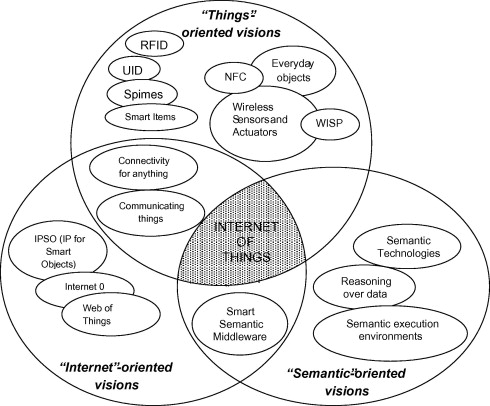
\includegraphics[width=\textwidth]{iot_visions}
  \caption{Internet of Things paradigmet ud fra tre visioner. Fra \cite{iot_survey_2010}.}
  \label{fig:iot_visions}
\end{figure}

\subsection{RFID}
RFID står for Radio Frequency IDentification, og som navnet antyder kan teknologien identificere objekter ved hjælp af radio frekvenser. Et RFID-tag, er en lille chip der indeholder en antenne, og en lille mængde data. Et objekt med et RFID-tag er nu \enquote{tagget}, og data om objektet kan læses ved hjælp af en RFID læser. Man kategoriserer typisk RFID-tags i passive og aktive. Et aktivt RFID-tag kræver strøm for at blive læst, og er derfor ofte tilsluttet et batteri. Et passivt RFID-tag kræver ingen strøm fra et batteri, men får derimod strømmen fra RFID-læseren \cite{want2006rfid}.

\subsection{Anvendelse af Internet of Things på Vestre Bådehavn}
\label{sub:iot_vestre_baadehavn}

Som beskrevet i \cref{sub:iot_koncept}, er der mange muligheder for hvilke sensorer der kan benyttes til at identificere objekter. Dette afsnit vil se på RFID og ultralyds sensorer, samt kameraer med billedgenkendelses software, som mulige sensorer, der kan benyttes på en havn som Vestre Bådehavn.

Lad os antage at alle både er blevet tagget med passive RFID-tags, sådan at de hver har en unik identifikation. Passive RFID-tags vægles da de er billige, og kan sidde på både uden nogen direkte afhængighed af elektricitet. Derudover kan hver vandlejeplads registrere, ved hjælp af en sensor, hvorvidt vandlejepladsen er optaget. Hvis der ligger en båd, kan en anden sensor også se hvem der ejer båden.

Sensoren som registrerer hvorvidt der ligger en båd på en vandlejeplads, kunne være en ultralyds sensor. Denne kan ved hjælp af lydbølger detektere tilstedeværelse af et objekt. Den kan dog ikke med stor præcision identificere objektet. En anden løsning er et kamera der ved hjælp af billed genkendelse kan identificere båden.

En computer forbundet til disse to typer sensorer, kan nu effektivt administrere en kæmpe havn med mange vandlejepladser. Når en ny båd lægger til på en vandlejeplads, vil computeren med det samme vide dette. Computeren kan derudover også kategorisere båden som en medlemsbåd eller som en gæstebåd. Da computeren nu har registreret at vandlejepladsen er optaget, skal den vende et skilt eller tænde for en diode, eller på anden måde ændres pladsens status til optaget.


\subsection{Opsummering}

I dette projekt arbejdes der udelukkende på en software løsning, og ikke på implementering af hardware. Derfor vil sensorerne som skal registrere bådene i havnen, blot blive simuleret, da deres tekniske opbygning ikke er direkte relevant for implementeringen af software løsningen. 

De simulerede sensorer kan opfatte tre tilstande. Enten kan den registrere at der ligger en ukendt båd, en kendt båd, eller ingen båd. Den ukendte båd vil være en gæst, og den kendte båd et medlem. Når en sensor opfanger et skift fra én tilstand til en anden, vil den sende et signal til softwareløsningen med info om den nye tilstand.

Det vurderes, på baggrund at den stigende interesse for \enquote{Internet of Things}, at denne slags sensorer er en del af en realistisk fremtidshorisont. Dette er en væsentlig forudsætning for den følgende løsningsmodels udgangspunkt.


%!TEX root = ../../Master.tex
\section{Usecases}

\subsection{Usecases:}

\begin{itemize}
  \item Gæst vil finde en plads:
  \begin{itemize}
    \item 1) Ny gæst melder til systemet, hvor lang tid han vil ligge til.
    \item 2) Systemet returnerer en liste over pladser som vil passe hans behov.
    \item 3) Gæsten vælger en plads som passer til hans båd.
    \item 4) Systemet melder at pladsen er nu reserveret (rød lampe).
    \item 5) Gæsten betaler for pladsen.
    \item 6) Systemet melder til havnefogeden at der er nye ankomne.

    \item Alternativ: De tre første 2 skridt er ikke nødvendige.
  \end{itemize}

  \item Medlem forlader sin plads:
  \begin{itemize}
    \item 1) Medlemmer melder til systemet tidspunkt for afrejse og hjemkomst.
    \item 2) Systemet venter til efter afrejse tidspunktet.
    \item 3) Når pladsen tømmes, da melder systemet at pladsen er fri (grøn lampe).
  \end{itemize}

  \item Medlem vender tilbage til sin plads:
  \begin{itemize}
    \item 1) Systemet registrerer når medlemmet ligger til, og melder at plads er optaget (rød lampe).
  \end{itemize}

  \item Havnefogeden melder plads optaget:
  \begin{itemize}
    \item 1) Medlem ringer til havnefogeden og fortæller om tidlig hjemkomst.
    \item 2) Havnefogeden indtaster (ny) dato i systemet.
    \item 3) Systemet returnere enten a eller b
    \item a) Dato er accepteret
    \item 1b) En gæst har lejet pladsen for en længere periode.
    \item 2b) Systemet foreslår en ny plads til gæsten.
    \item 3b) Havnefogeden snakker med gæsten.
  \end{itemize}

  \item Automatisk arrangementsforslag:
  \begin{itemize}
    \item 1) Antallet af medlemmer i havnen overstiger et bestemt niveau.
    \item 2) Systemet melder at det ville være en god dag for et arrangement.
    \item 3) Et medlem af klubben ser denne melding, og foreslår et arrangement.
  \end{itemize}

  \item Automatisk medlemstjek
  \begin{itemize}
    \item 1) Systemet registrerer uoverensstemmelse med angivet rejseplan.
    \item 2) Systemet notificerer havnefogeden omkring overensstemmelsen.
  \end{itemize}
  

\end{itemize}



\section{Systematisk Test af Program}
\label{sec:systematisk_test_af_program}

\subsection{Test Driven Development}
\label{sub:test_driven_development}

For at sikre at programmet er let at teste, er kernefunktionerne i programmet udviklet jævnfør softwareudviklingsprocessen \enquote{Test Driven Development}. I Test Driven Development (TDD) skrives unit tests af en metode, før selve implementeringen af funktionen. Denne udviklingsprocess sikrer, at nye funktionaliteter ikke ødelægger de forud eksisterende \cite{martin2006agile}. Programmøren tvinges også til at tænke på, hvordan metoden bruges ved kald. Det sikres hermed, at metoden er overskueligt konstrueret, således at den kan kaldes uden unødigt besvær. Et andet aspekt af TDD, er at testkoden tjener som dokumentation af den testede metodes funktionalitet. Tilgengæld riskeres et øget tidsforbrug, der dog muligvis kan fraskrives fejlfinding.

\subsection{Unit Testing i Microsoft Visual Studio}
\label{sub:unit_testing_i_microsoft_visual_studio}

Microsofts unit test framework for managed code er anvendt til unit testing. Frameworket kan teste \enquote{managed code}, som C\# falder ind under. Når tests er skrevet, kan Test Explorer i Visual Studio køre testene. Når testene er færdige, vil resultaterne blive præsenteret som failed tests, passed tests, not run tests og skipped tests \cite{msdn_unittest}.

Før der skrives unit tests, skal der oprettes et unit test projekt. Herefter kan der tilføjes klasser annoteret med \enquote{[TestClass]}. Inde i disse klasser, tilføjer man de metoder, annoteret med \enquote{[TestMethod]}, som skal køres. Et eksempel på en test metode, kan se i \cref{lst:test_notfound}.
Alle tests til systemet kan findes på CD'en der afleveres som bilag.

\begin{lstlisting}[label=lst:test_notfound, caption={Eksempel på testfunktion}]
  [TestMethod]
  public void ShouldThrowWhenNotFound()
  {
      var space = new WaterSpace(404404, 4.3, 5.4);
      try
      {
          var test = BoatDetector.BoatAt(space);
      }
      catch (KeyNotFoundException _)
      {
          return;
      }
      Assert.Fail("No exception was thrown.");
  }
\end{lstlisting}



\begin{figure}
  \centering
  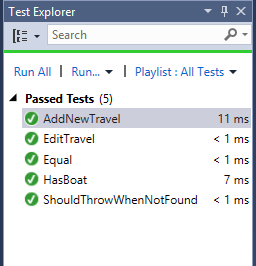
\includegraphics{test_explorer.png}
  \caption{Resultat af tests i Test Explorer i Visual Studio 2013}
  \label{fig:test_explorer}
\end{figure}


\section{Håndtering af Brugertilladelser} % (fold)
\label{tilladelser}

De forskellige aktører for systemet, har forskellige niveauer af tilladelser i havnen. Eksempelvis skal havnefogeden have adgang til at se alle medlemmernes rejser, i modsætning til et menigt medlem, der kun har adgang til at se sine egne rejser. For at kunne korrekt modellere de administrative ansvarsområder, er det nødvendigt at kunne skelne i mellem brugere, og deres tilladelser.

Der findes tre grader af brugertilladelse, ingen, læse eller skrive. Graden \enquote{ingen}, er den laveste grad, og betyder at den respektive bruger ikke har nogen som helst form for adgang til de pågældende datafelt. Graden \enquote{læse} gør datafeltet synligt for brugeren. Graden \enquote{skrive} giver brugeren mulighed for at redigere datafeltet. Brugertilladelser er akkumulerende, således at skrivetilladelsen implicit også er en læsetilladelse. 

Alle brugere har for ethvert datafelt én af de tre grader af brugertilladelser. Dette giver mulighed for at differentierer imellem forskellige instanser af brugermodellen, således at det ikke er nødvendigt at oprette en ny brugermodel, for enhver kombination af brugertilladelser.

Brugere tilgår systemet via et chipkort, som indeholder information der kan identificere brugeren data i systemet. Det er også muligt for medlemmer at tilgå systemet via deres medlemsnummer og et kodeord.

Når en bruger tilgår systemet, bliver programmet initialiseret, ud fra de tilladelser brugeren har. Synligheden bliver på denne måde begrænset, således at al information ikke er frit tilgængeligt, samt at brugergrænsefladen holdes så relevant som muligt.

\kanote{kodeeksempler  + forudgående tekst}

\kanote{husk mulighed for ny gæst}

\section{Klasse Design}
\label{sec:klasse_design}
Som beskrevet i \cref{sec:klasse_teori} er det vigtig at få lave klassehierarkiet så det modelere de ting fra virkeligheder som programmet håndtere. Denne sektion vil dokumenter de grundlæggende modeller, som programmet er bygget op efter. 

For at give et overblik over klassehierarkiet er der lavet et UML-klassediagram som ses på \cref{fig:UML}. På diagrammet kan man se de vigtigste klasser der er brugt i løsningen. Af diagrammet fremgår også klassernes relationer.

De følgende under sektion beskriver programmets primære klasser og hvilken data som er inderholdt i klasserne.


\begin{figure}
  \centering
  \vspace*{-4.5cm}
  \makebox[\textwidth]{
    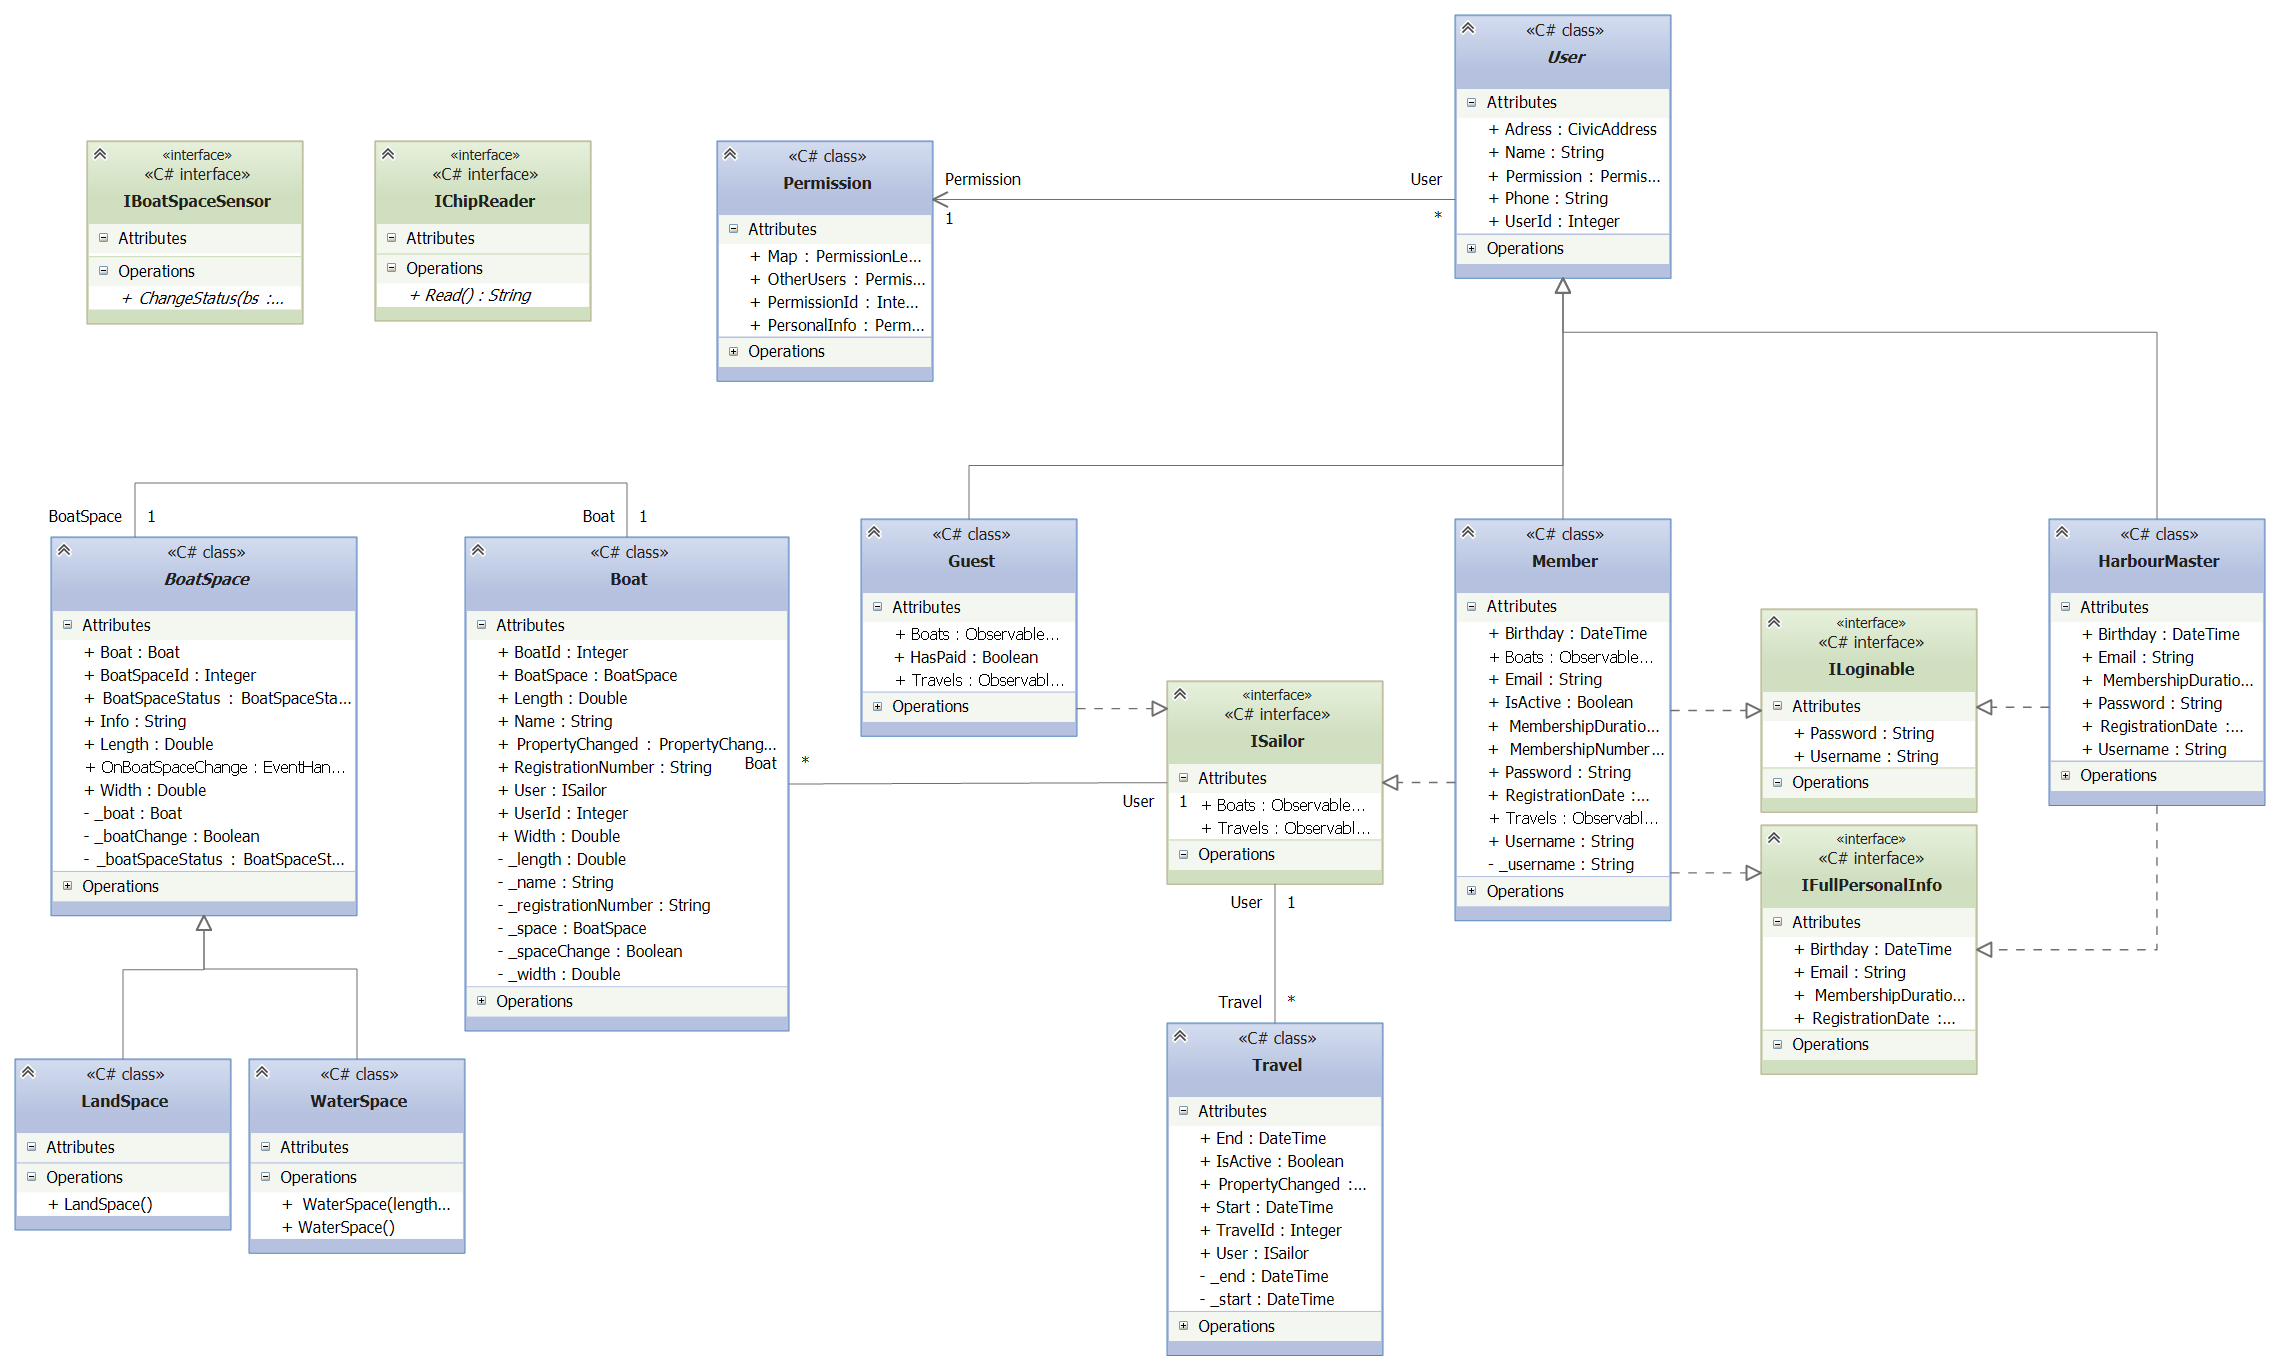
\includegraphics[width=1.2\paperwidth, angle = 270]{UML.png}
  }
 	\caption{UML-klassediagram over klasser der bruges til at modellere løsningen.} \label{fig:UML}  
 \end{figure}

\alnote{skriv om de to ensomme interfaces}

\subsection{Modellering af Brugere}
\label{sub:brugere_af_programmet}

I klassehierarkiets top ligger den abstrakte klasse \enquote{User}. En \enquote{User} er en generel bruger af systemet. Denne klasse definerer alle fællestræk de nedarvende klasser skal have. Dette inkluderer brugerrettigheder og basale informationer som telefonnummer, navn og adresse. Der findes tre forskellige interfaces, der indeholder forskellige informationer om brugere: \enquote{IFullPersonalInfo}, \enquote{ISailor}, \enquote{ILoginable}.

Subklasserne til \enquote{User} opdeler brugere som enten medlemmer af klubben, gæster eller havnefoged. Til disse tre brugertyper bruges klasserne \enquote{HarbourMaster}, \enquote{Guest} og \enquote{Member}. Denne opdeling er lavet fordi der indgår forskellige felter på tværs af disse subklasser, og de tre brugertyper er helt forskellige kategorier i programmet. 

For at differentiere subklasserne, implementeres forskellige kombinationer af interfaces. Eksempelvis må en havnefoged ikke have en båd, og derfor implementerer klassen \enquote{HarbourMaster} ikke \enquote{ISailer} interfacet. Til gengæld deler \enquote{HarbourMaster}, \enquote{IFullPersonalInfo} og \enquote{ILoginable} med \enquote{Member} klassen, da de begge har behov for at gemme mere personinformation, samt at kunne logge ind med brugernavn/medlemsnummer.
 
\subsection{Modellering af Rejser}
\label{sub:rejser}

En medlems rejse modelleres med klassen \enquote{Travel}. Den indeholder information om rejsen start- og slutdato. \enquote{Travels} bruges også til at angive hvor lang tid en gæst ligger i havnen. \enquote{Travel} implementere \enquote{IEquatable} interfacet, som gør det muligt at sammenligne med andre klasser af samme type. Klasser der implementere ISailor indeholder en liste af \enquote{Travels}.
 
\subsection{Modellering af Både}
\label{sub:bade}

Der er lavet en klasse til både, der hedder \enquote{Boat}. Denne klasse bruges til at gemme data tilhørende en båd. Der gemmes dens navn og størrelse, så man kan tjekke hvorvidt en given plads er stor nok til at rumme båden.

\subsection{Modellering af Bådpladser}
\label{sub:pladser}

Der er to klasser til repræsentation af bådpladser. Klassen \enquote{WaterSpace} modellere vandpladser og \enquote{LandSpace} modellere landplads. Begge disse klasser nedarver fra klassen \enquote{BoatSpace}, som indeholder generelle informationer om en bådplads. 

\subsection{associationer}
\label{sub:associationer}

I klassehierarkiet benyttes to typer associationer binær associationer og en-til-mange associationer. Den binære association på \cref{fig:UML} mellem både og bådpladser viser at der er en reference inderhold i båden til dens tilhørende bådplads, og vise versa. Denne association håndter at en båd tildeles en plads, får samme plads også tildelt en reference til båden. Association sikker derved også at man ikke kan tildele en plads en båd, hvis pladsen allerede inderholde en reference til en anden båd. 

En ISailor indeholder en liste til boats og en liste til Travels, mens Travels og både kun inderholder en reference til en ISailor. Dette udgør en én-til-mange association fra ISailor til boats. Denne association sikre at tilføjes et objekt til en liste inderholdt i en ISailor, tildeles objektet automatisk en reference til samme ISailor. Hvis en båd får tildelt en ISailor som sin ejer, tilføjes båden også til listen af ejerens Både. 





\subsection{Database}
\label{sub:database}





\section{Reflection}
\label{sec:reflection}

Reflection er en metode i C\# til at undersøge objekter i et program ved kørselstid. Et eksempel på brugen af reflection kan være, at programmøren ønsker at finde et felt i en klasse ved navn.

I dette projekt bruges reflection til at gøre metoder der tilgår databasen, meget generiske, hvilket sikrer stor kodegenbrug. Som beskrevet i \cref{sec:database}, består databasen af forskellige tabeller, herunder \enquote{Users}, \enquote{Boats}, \enquote{BoatSpaces} og \enquote{Travels}. Lad os forestille os en metode der skal slette et objekt fra en specifik tabel. Metodesignaturen for en sådan metode kunne se ud som vist i \cref{lst:reflection_remove1}.


\begin{lstlisting}[label=lst:reflection_remove1]
public void RemoveUser(User user)
\end{lstlisting}

Problemet med denne metode er at denne metode kun virker på \enquote{User} objekter. Dette betyder at der udover denne metode også skal skrives en \enquote{RemoveBoat}, \enquote{RemoveBoatSpace} og en \enquote{RemoveTravel} metode. For at undgå dette, kan der laves en \enquote{Remove} metode, med en parameter der afgør hvilken tabel der skal slettes noget i. Metodesignaturen kunne se ud som i \cref{lst:reflection_remove2}.


\begin{lstlisting}[label=lst:reflection_remove2]
public void Remove<T>(T item, string table)
\end{lstlisting}

Problemet er, at metoden \enquote{Remove} skal have \enquote{hard-codet} alle de forskellige navne på alle eksisterende tabeller ind i denne metode. Hvis navnet på en tabel så ændrer sig, vil metoden ikke længere virke.

For at løse ovenstående problemer kommer reflection ind i billedet. \Cref{lst:reflection_verifytable} er et kodeeksempel fra programmet, som leder efter en property der er af typen \enquote{DbSet<T>}, hvor T er en generisk type. Først finder metoden alle properties der er defineret på typen \enquote{LobobContext}. DBsetType er den property der ønskes fundet. Metoden itererer nu alle properties igennem, indtil en property der matcher DBsetType er fundet. Hvis der er ingen matches, findes den ønskede tabel ikke, og null returneres. Hvis der er et match i foreach løkken, findes property navnet, og lægges over i dbSetTarget. Det er nu muligt at dynamisk oprette en DbSet<T> ud fra typen \enquote{LobobContext}. Denne DbSet<T> returneres, og kan nu bruges i en \enquote{Remove} metode.

\begin{lstlisting}[label=lst:reflection_verifytable]
private DbSet<T> VerifyTable<T>(LobopContext context) where T : class
{
    Type lobobContextType = typeof(LobopContext);
    PropertyInfo[] properties = lobobContextType.GetProperties();
    Type DBsetType = typeof(DbSet<T>);
    string dbSetTarget = string.Empty;

    foreach (PropertyInfo item in properties)
    {
        if (DBsetType == item.PropertyType)
        {
            // table found
            dbSetTarget = item.ToString().Split(' ')[1];
            DbSet<T> dbSet = (DbSet<T>)lobobContextType.GetProperty(dbSetTarget).GetValue(context, null);
            return dbSet;
        }
    }
    // table of type not found
    return null;
}
\end{lstlisting}

Den færdige Remove metode der er generisk, virker nu på tværs af alle klasser, ved hjælp af reflection. Hvis en Titanic båden skal fjernes fra \enquote{Boats} tabellen, kaldes koden set i \cref{lst:reflection_remove3}. Der er nu ingen behov for at specificere i hvilken tabel titanic skal fjernes fra, da Remove selv kan regne dette ud udfra den generiske typeparameter <Boat>.

\begin{lstlisting}[label=lst:reflection_remove3]
Remove<Boat>(titanic);
\end{lstlisting}



%\section{Om Systemet}
\label{sec:om_systemet}

Systemet der omtales i \cref{cha:problemformulering} tænkes at være en konsolapplikation skrevet i C\#. Programmet interagerer med en database. Denne databse gemmer alle informationer der er tilgængelige gennem programmet.

\subsection{Eksempler På Kommandoer}
\label{sub:eksempler_p_kommandoer}

Da systemet giver mulighed for at håndtere gæster, skal det være muligt at tildele en gæst til en given vandlejeplads. Nedenstående \cref{lst:add_guest} tilføjer en gæst til databasen, fortæller at han holder ved vandlejeplads 42, hedder Jens Jensen og at han har betalt indtil 1. juni 2014.

\begin{lstlisting}[language=bash, label=lst:add_guest] 
  $ program add guest --boatarea=42 --name="Jens Jensen" --until="1/6/2014" 
\end{lstlisting}


